\section{MÔ HÌNH MẠNG CAMPUS ĐỀ XUẤT}\label{sec:mo_hinh_de_xuat}

Chương này trình bày thiết kế hệ thống: yêu cầu, kiến trúc, sơ đồ vật lý và sơ đồ logic, quy hoạch địa chỉ, định tuyến, SDN, SD-WAN, dịch vụ và bảo mật. Mọi thông số thống nhất với cấu hình đang vận hành của thiết bị.

\subsection{Phân tích bài toán và yêu cầu thiết kế}

Đề tài giả định một trường đại học có cơ sở chính và ba cơ sở phụ tại Cần Thơ, Đà Nẵng, Nha Trang. Cơ sở chính có các khoa Công nghệ thông tin, Toán -- Thống kê, Luật, khối Hành chính và toàn bộ dịch vụ dùng chung; mỗi cơ sở phụ có hai khối nghiệp vụ và cần dùng dịch vụ tại cơ sở chính. Mạng truyền thống bộc lộ ba vấn đề khi quy mô tăng: thay đổi chính sách phải làm trên nhiều thiết bị; không có cái nhìn toàn cục về lớp 2; WAN phụ thuộc một đường truyền. Bài toán đặt ra là điều khiển tập trung mạng nội bộ cơ sở chính bằng SDN, nối các cơ sở bằng overlay SD-WAN trên hai nhà cung cấp độc lập, đồng thời giữ VRRP, OSPF và tường lửa HA tại những vị trí cần độ ổn định cao.

\textbf{Yêu cầu chức năng:} máy trạm mọi cơ sở dùng được dịch vụ dùng chung; mỗi khoa/khối là một VLAN và một subnet, tách riêng vùng máy chủ, DMZ và quản trị; máy trạm nhận địa chỉ qua DHCP; DNS nội bộ \texttt{campus.internal}, Web HTTPS, Mail và Syslog; Controller quản lý toàn bộ switch lớp 2 cơ sở chính, chống vòng lặp, chặn cổng tập trung, có REST API và giám sát tải; Edge được xác thực bằng chứng thư, overlay IPsec trên hai transport, chính sách SLA/AAR và lọc tập trung; tường lửa chỉ mở dịch vụ cần thiết; người dùng ra Internet tại chỗ có dự phòng; giám sát và tự động cảnh báo sự cố WAN.

\textbf{Yêu cầu phi chức năng:} không có điểm lỗi đơn tại gateway, lõi, biên, WAN và lớp 2; quy tắc địa chỉ thống nhất theo site để thêm cơ sở mới chỉ cần cấp Site-ID, System-IP, subnet và dùng lại khuôn cấu hình; quản trị tập trung qua ASDM, vManage và Controller; mỗi thiết bị có định danh, địa chỉ và vai trò rõ ràng.

\subsection{Kiến trúc tổng thể}

Hệ thống gồm sáu site và hai miền truyền tải (Bảng~\ref{tab:cac_site}).

\begin{table}[H]
    \centering
    \small
    \caption{Các site và vai trò trong mô hình}
    \label{tab:cac_site}
    \begin{tabularx}{\textwidth}{|c|L{3.4cm}|c|Y|}
        \hline
        \textbf{Site-ID} & \textbf{Tên} & \textbf{ASN} & \textbf{Thành phần chính} \\
        \hline
        100 & Campus chính & 65000 & Cặp ASAv HA, Core-SW1/2, Dist-SW1/2 và Access-SW1--4 (OVS), SDN Controller (Ryu), Server Farm, DMZ, hai vEdge \\
        \hline
        200 & Cơ sở Cần Thơ & 65010 & Brand-FW, SwitchBrand, hai switch khối, hai vEdge; VLAN 60, 70 \\
        \hline
        300 & Cơ sở Đà Nẵng & 65020 & Như Site 200; VLAN 80, 90 \\
        \hline
        400 & Cơ sở Nha Trang & 65030 & Như Site 200; VLAN 50, 60 \\
        \hline
        500 & Cơ sở mở rộng & 65040 & Hai vEdge, Brand-FW-S500, SW-S500, hai máy trạm \\
        \hline
        900 & Trung tâm điều khiển SD-WAN & -- & vManage, vSmart, vBond, switch LAN, switch quản trị, máy trạm quản trị \\
        \hline
        -- & Nhà cung cấp Internet & 64511 & Router vIOS, color \texttt{biz-internet}; nối ra mạng thật của phòng lab \\
        \hline
        -- & Nhà cung cấp MPLS & 64512 & Router vIOS, color \texttt{mpls} \\
        \hline
    \end{tabularx}
\end{table}

Kiến trúc có ba mặt phẳng: \textbf{dữ liệu} (switch, tường lửa, Edge, router nhà cung cấp); \textbf{điều khiển} gồm hai miền độc lập --- SDN Controller điều khiển lớp 2 cơ sở chính qua OpenFlow 1.3 trên VLAN 99 và vSmart điều khiển overlay qua OMP, còn lớp 3 cơ sở chính vẫn dùng OSPF, VRRP phân tán; \textbf{quản trị} gồm VLAN 99 tại cơ sở chính và mạng \texttt{10.9.0.0/24}, \texttt{10.9.1.0/24} tại Site 900. Nguyên tắc phân vai: Core chỉ định tuyến liên VLAN và làm gateway; OVS chỉ chuyển mạch lớp 2 theo flow của Controller; tường lửa kiểm soát biên và DMZ; vEdge làm router WAN và đầu cuối overlay; tường lửa chi nhánh kiêm gateway và DHCP.

\subsection{Sơ đồ vật lý và sơ đồ logic}\label{sec:so_do}

\textbf{Sơ đồ vật lý} (Hình~\ref{fig:kien_truc_tong_the_campus}) thể hiện toàn bộ thiết bị và đấu nối cổng của hệ thống trên EVE-NG: 74 node, 107 phân đoạn mạng, nhãn cổng và địa chỉ giao diện.

\begin{figure}[H]
    \centering
    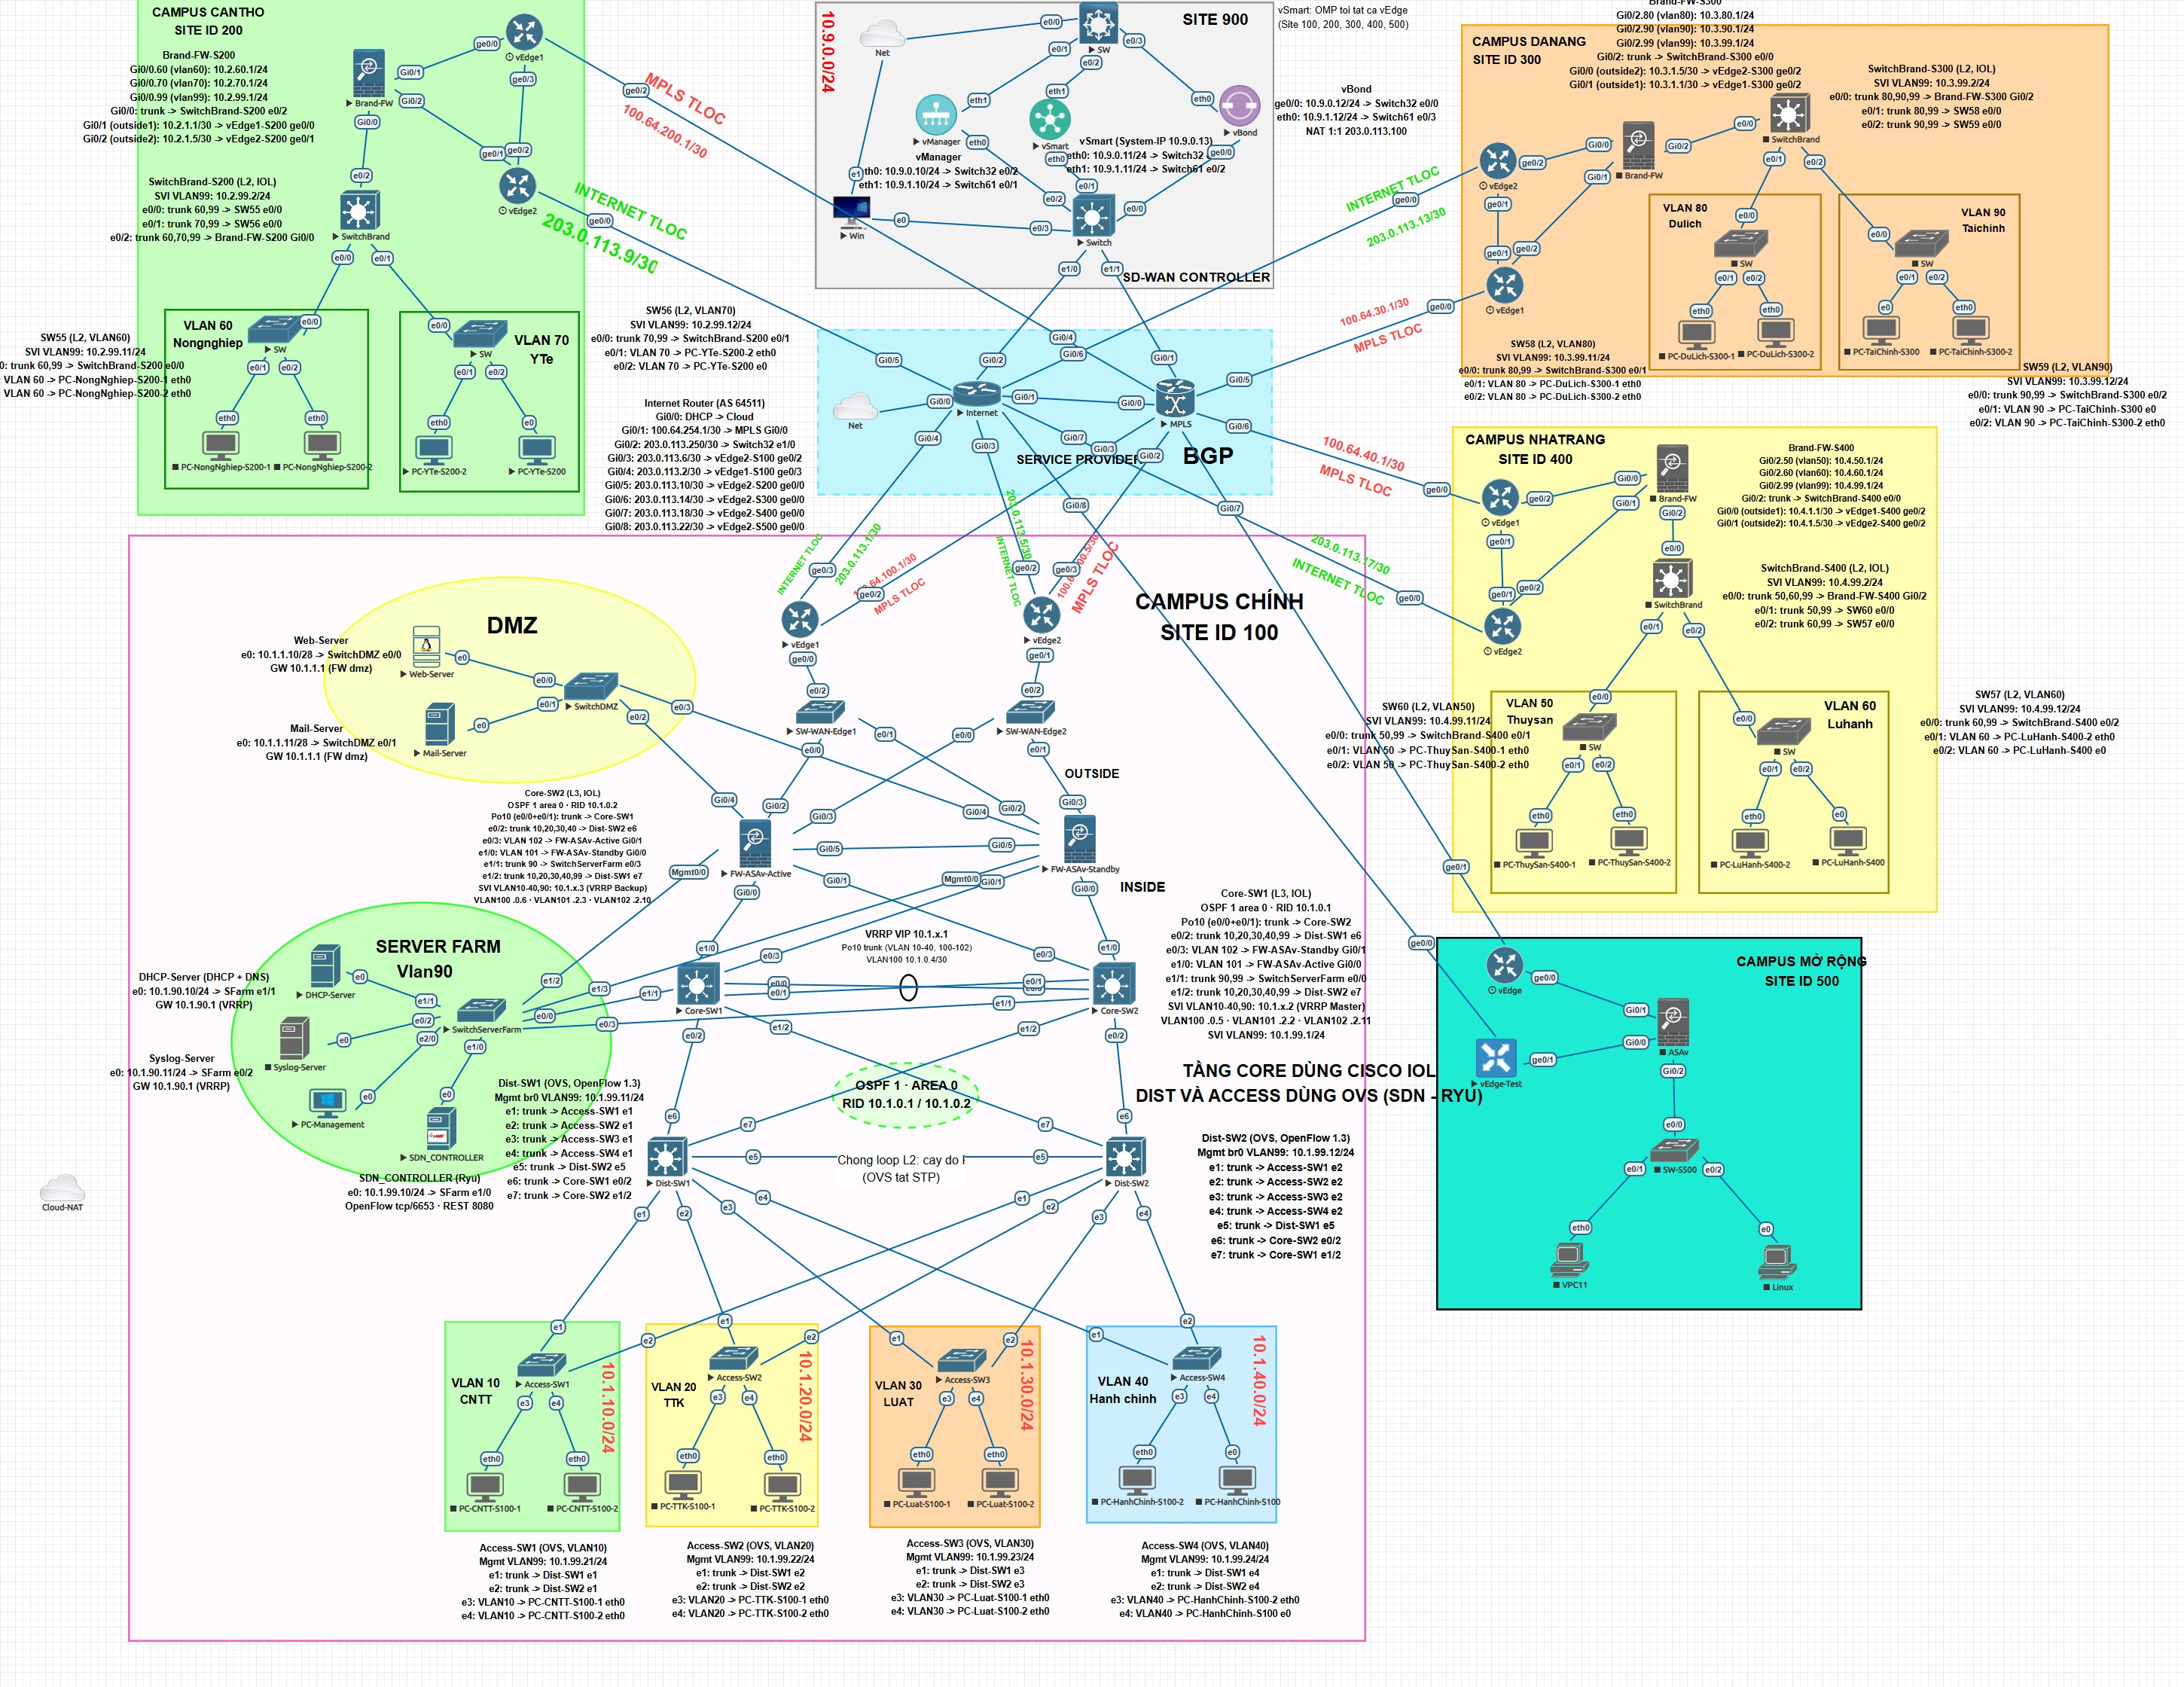
\includegraphics[width=\textwidth]{image/topo-vatly.jpg}
    \caption{Sơ đồ vật lý của hệ thống trên EVE-NG}
    \label{fig:kien_truc_tong_the_campus}
\end{figure}

\textbf{Sơ đồ logic} (Hình~\ref{fig:so_do_logic}) thể hiện hệ thống ở lớp 3: subnet và gateway của từng VLAN, các mạng transit, miền định tuyến (OSPF Area~0 tại Campus chính, eBGP underlay với hai nhà cung cấp, OMP và overlay IPsec giữa các Edge) và vị trí các dịch vụ.

\begin{figure}[H]
    \centering
    \resizebox{\textwidth}{!}{%
    \begin{tikzpicture}[
        font=\scriptsize, >=stealth,
        box/.style={draw, rounded corners=2pt, align=center, line width=0.7pt, inner sep=3pt},
        s100/.style={box, fill=blue!5, draw=blue!60!black, text width=6.0cm},
        br/.style={box, fill=teal!5, draw=teal!60!black, text width=6.4cm},
        tr/.style={box, fill=gray!12, draw=black!70, text width=3.0cm},
        ctl/.style={box, fill=purple!7, draw=purple!70!black, text width=9.0cm},
        inet/.style={draw=blue!75!black, line width=1.1pt},
        mpls/.style={draw=orange!85!black, line width=1.1pt},
        lan/.style={line width=0.8pt, black!70},
        lbl/.style={font=\tiny, fill=white, inner sep=1pt, align=center}
    ]
        % Site 900 va hai nha cung cap
        \node[ctl] (s900) at (0.4,9.6) {\textbf{Site 900 -- Controller LAN \texttt{10.9.0.0/24}} (gateway switch LAN \texttt{.2})\\
            vManage \texttt{.10} \textperiodcentered{} vSmart \texttt{.11} \textperiodcentered{} vBond \texttt{.12} \textperiodcentered{} mặt quản trị \texttt{10.9.1.0/24}\\
            Tuyến tĩnh CE--PE tới hai nhà cung cấp; ra Internet có kiểm soát};
        \node[tr] (inet) at (-2.5,7.6) {\textbf{Internet} -- AS 64511\\\texttt{203.0.113.0/24}\\color \texttt{biz-internet}};
        \node[tr] (mpls) at (3.3,7.6) {\textbf{MPLS} -- AS 64512\\\texttt{100.64.0.0/10}\\color \texttt{mpls}};
        \draw[black!70, line width=0.8pt] (inet) -- node[lbl]{eBGP\\\texttt{100.64.254.0/30}} (mpls);
        \draw[inet] (s900.south -| inet.north) -- (inet.north);
        \draw[mpls] (s900.south -| mpls.north) -- (mpls.north);

        % Hai duong truc transport
        \draw[inet] (inet.south) -- (-2.5,6.5) -- (-0.1,6.5) -- (-0.1,-4.2);
        \draw[mpls] (mpls.south) -- (3.3,6.3) -- (0.7,6.3) -- (0.7,-4.2);

        % Site 100
        \node[s100] (ve) at (-4.3,5.3) {\textbf{vEdge1/2-S100} -- AS 65000\\System-IP \texttt{10.200.100.1}, \texttt{10.200.100.2}\\mỗi vEdge hai TLOC; NAT ra Internet (DIA)\\VPN 1: beacon \texttt{10.1.255.1/32}};
        \node[s100] (fw) at (-4.3,3.05) {\textbf{FW-ASAv HA} (Active/Standby)\\outside \texttt{10.1.3.0/29}, outside2 \texttt{10.1.3.8/29}\\DMZ \texttt{10.1.1.0/28}: Web \texttt{.10}, Mail \texttt{.11}};
        \node[s100] (core) at (-4.3,1.2) {\textbf{Core-SW1/2}: SVI, VRRP VIP \texttt{.1}, DHCP Relay\\transit \texttt{10.1.2.0/29}, \texttt{10.1.2.8/29}\\Po10 \texttt{10.1.0.4/30}};
        \node[s100] (vl) at (-4.3,-1.05) {VLAN 10 \texttt{10.1.10.0/24} -- CNTT\\VLAN 20 \texttt{10.1.20.0/24} -- Toán-TK\\VLAN 30 \texttt{10.1.30.0/24} -- Luật\\VLAN 40 \texttt{10.1.40.0/24} -- Hành chính\\VLAN 90 \texttt{10.1.90.0/24} -- DHCP/DNS \texttt{.10}, Syslog \texttt{.11}\\VLAN 99 \texttt{10.1.99.0/24} -- quản trị, Controller \texttt{.10}};
        \node[s100, fill=green!7, draw=green!45!black] (sdn) at (-4.3,-3.35) {\textbf{Khối SDN lớp 2}: 6 OVS\\Ryu điều khiển qua OpenFlow 1.3 trên VLAN 99};
        \draw[lan] (ve) -- node[lbl, right=1pt]{OSPF Area 0 (VPN 1)} (fw);
        \draw[lan] (fw) -- node[lbl, right=1pt]{OSPF Area 0} (core);
        \draw[lan] (core) -- node[lbl, right=1pt]{SVI} (vl);
        \draw[lan] (vl) -- node[lbl, right=1pt]{trunk 802.1Q} (sdn);
        \begin{scope}[on background layer]
            \node[draw=blue!60!black, dashed, rounded corners, fill=blue!2, fit=(ve)(sdn), inner sep=5pt] (s100box) {};
        \end{scope}
        \node[font=\scriptsize\bfseries, blue!60!black, anchor=south west] at (s100box.north west) {Site 100 -- Campus chính, \texttt{10.1.0.0/16}};
        \draw[inet] ([yshift=2mm]ve.east) -- ([yshift=2mm]ve.east -| -0.1,0);
        \draw[mpls] ([yshift=-2mm]ve.east) -- ([yshift=-2mm]ve.east -| 0.7,0);

        % Chi nhanh
        \node[br] (b200) at (5.0,5.2) {\textbf{Site 200 -- Cần Thơ}, AS 65010, \texttt{10.2.0.0/16}\\vEdge1 \texttt{10.200.200.1} (mpls)\\vEdge2 \texttt{10.200.200.2} (biz-internet)\\Brand-FW: \texttt{10.2.1.0/30}, \texttt{10.2.1.4/30}\\VLAN 60 \texttt{10.2.60.0/24}, VLAN 70 \texttt{10.2.70.0/24}};
        \node[br] (b300) at (5.0,2.55) {\textbf{Site 300 -- Đà Nẵng}, AS 65020, \texttt{10.3.0.0/16}\\vEdge1 \texttt{10.200.30.1} (mpls)\\vEdge2 \texttt{10.200.30.2} (biz-internet)\\Brand-FW: \texttt{10.3.1.0/30}, \texttt{10.3.1.4/30}\\VLAN 80 \texttt{10.3.80.0/24}, VLAN 90 \texttt{10.3.90.0/24}};
        \node[br] (b400) at (5.0,-0.1) {\textbf{Site 400 -- Nha Trang}, AS 65030, \texttt{10.4.0.0/16}\\vEdge1 \texttt{10.200.40.1} (mpls)\\vEdge2 \texttt{10.200.40.2} (biz-internet)\\Brand-FW: \texttt{10.4.1.0/30}, \texttt{10.4.1.4/30}\\VLAN 50 \texttt{10.4.50.0/24}, VLAN 60 \texttt{10.4.60.0/24}};
        \node[br] (b500) at (5.0,-2.75) {\textbf{Site 500 -- cơ sở mở rộng}, AS 65040, \texttt{10.5.0.0/16}\\vEdge1 \texttt{10.200.50.1} (mpls)\\vEdge2 \texttt{10.200.50.2} (biz-internet)\\Brand-FW-S500: \texttt{10.5.1.0/30}, \texttt{10.5.1.4/30}\\VLAN 10 \texttt{10.5.10.0/24}};
        \foreach \b in {b200,b300,b400,b500} {
            \draw[mpls] ([yshift=2mm]\b.west) -- ([yshift=2mm]\b.west -| 0.7,0);
            \draw[inet] ([yshift=-2mm]\b.west) -- ([yshift=-2mm]\b.west -| -0.1,0);
        }

        \node[align=center, font=\scriptsize, text width=14.5cm] at (0.4,-4.85) {\textcolor{blue!75!black}{\rule[0.5ex]{0.9cm}{1.1pt}} Internet (eBGP, \texttt{203.0.113.x/30}) \qquad
            \textcolor{orange!85!black}{\rule[0.5ex]{0.9cm}{1.1pt}} MPLS (eBGP, \texttt{100.64.x.x/30})\\
            Overlay IPsec full-mesh giữa các TLOC, OMP tới vSmart, BFD trong mỗi đường hầm. Gateway mọi VLAN là \texttt{.1}; VLAN 99 quản trị có ở mọi site};
    \end{tikzpicture}%
    }
    \caption{Sơ đồ logic của hệ thống: subnet, gateway và miền định tuyến}
    \label{fig:so_do_logic}
\end{figure}

\subsection{Thiết kế chi tiết từng site}

\subsubsection{Campus chính (Site 100)}

Hình~\ref{fig:topology_site100} là sơ đồ đấu nối chi tiết Campus chính.

\begin{figure}[H]
    \centering
    \resizebox{0.92\textwidth}{!}{%
    \begin{tikzpicture}[
        font=\small, >=stealth,
        dev/.style={draw, rounded corners=2pt, align=center, minimum height=1.1cm, text width=3.3cm, line width=0.8pt, font=\linespread{1}\small},
        wan/.style={dev, fill=gray!10, draw=black!70},
        edge/.style={dev, fill=red!5, draw=red!60!black},
        fw/.style={dev, fill=orange!8, draw=orange!70!black},
        l2/.style={dev, fill=blue!4, draw=blue!50!black},
        core/.style={dev, fill=blue!10, draw=blue!65!black},
        ovs/.style={dev, fill=green!7, draw=green!40!black, text width=3.5cm},
        srv/.style={dev, fill=yellow!8, draw=yellow!45!black},
        lbl/.style={font=\footnotesize, fill=white, inner sep=1.5pt},
        act/.style={line width=1.1pt},
        stb/.style={dashed, line width=0.7pt, black!60}
    ]
        \node[wan] (inet) at (-3.5,17.0) {\textbf{Internet}\\AS 64511};
        \node[wan] (mpls) at (3.5,17.0) {\textbf{MPLS}\\AS 64512};
        \node[edge] (ve1) at (-6.8,15.2) {\textbf{vEdge1-S100}\\System-IP 10.200.100.1};
        \node[edge] (ve2) at (6.8,15.2) {\textbf{vEdge2-S100}\\System-IP 10.200.100.2};
        \node[l2] (swe1) at (-6.8,13.2) {\textbf{SW-WAN-Edge1}\\VLAN 103: 10.1.3.0/29};
        \node[l2] (swe2) at (6.8,13.2) {\textbf{SW-WAN-Edge2}\\VLAN 104: 10.1.3.8/29};
        \node[fw] (fwa) at (-6.8,9.8) {\textbf{FW-ASAv-Active}\\Primary (.1 / .9)};
        \node[fw] (fws) at (6.8,9.8) {\textbf{FW-ASAv-Standby}\\Secondary (.4 / .12)};
        \node[srv, text width=5.2cm] (dmz) at (0,9.45) {\textbf{DMZ} 10.1.1.0/28 (SwitchDMZ)\\Web-Server .10, Mail-Server .11};
        \node[core] (c1) at (-6.8,6.0) {\textbf{Core-SW1}\\VRRP Master, gốc cây};
        \node[core] (c2) at (6.8,6.0) {\textbf{Core-SW2}\\VRRP Backup};
        \node[srv, text width=5.2cm] (farm) at (0,5.3) {\textbf{SwitchServerFarm}\\VLAN 90: DHCP/DNS .10, Syslog .11\\VLAN 99: Controller .10,\\PC-Mgmt .50, FW Mgmt .33/.34};
        \node[ovs] (d1) at (-3,1.6) {\textbf{Dist-SW1} (OVS)};
        \node[ovs] (d2) at (3,1.6) {\textbf{Dist-SW2} (OVS)};
        \node[ovs] (a1) at (-7.8,-1.2) {\textbf{Access-SW1}\\VLAN 10 -- CNTT};
        \node[ovs] (a2) at (-2.6,-1.2) {\textbf{Access-SW2}\\VLAN 20 -- Toán-TK};
        \node[ovs] (a3) at (2.6,-1.2) {\textbf{Access-SW3}\\VLAN 30 -- Luật};
        \node[ovs] (a4) at (7.8,-1.2) {\textbf{Access-SW4}\\VLAN 40 -- Hành chính};

        \draw[act] (inet) -- (ve1); \draw[act] (inet) -- (ve2);
        \draw[act] (mpls) -- (ve1); \draw[act] (mpls) -- (ve2);
        \draw[act] (ve1) -- node[lbl]{OSPF} (swe1);
        \draw[act] (ve2) -- node[lbl]{OSPF} (swe2);
        \draw[act] (swe1) -- (fwa); \draw[stb] (swe1) -- (fws);
        \draw[act] (swe2) -- (fwa); \draw[stb] (swe2) -- (fws);
        \draw[act, orange!70!black] ([yshift=3.5mm]fwa.east) -- node[lbl, above=1pt]{failover Gi0/5} ([yshift=3.5mm]fws.west);
        \draw[act] (fwa.east |- dmz.west) -- node[lbl]{Gi0/4} (dmz.west);
        \draw[stb] (dmz.east) -- node[lbl]{Gi0/4} (fws.west |- dmz.east);
        \draw[act] (fwa) -- node[lbl]{VLAN 101} (c1);
        \draw[act] (fwa) -- node[lbl, pos=0.62]{VLAN 102} (c2);
        \draw[stb] (fws) -- node[lbl, pos=0.62]{VLAN 102} (c1);
        \draw[stb] (fws) -- node[lbl]{VLAN 101} (c2);
        \draw[act, blue!65!black] ([yshift=3.5mm]c1.east) -- node[lbl, above=1pt]{Po10 (LACP): VLAN 10--40, 100--102} ([yshift=3.5mm]c2.west);
        \draw[act] (c1.east |- 0,5.75) -- node[lbl]{VLAN 90, 99} (farm.west |- 0,5.75);
        \draw[act] (farm.east |- 0,5.75) -- node[lbl]{VLAN 90} (c2.west |- 0,5.75);
        \draw[act] (c1) -- node[lbl, pos=0.5]{D1-C1} (d1);
        \draw[act] (c1) -- node[lbl, pos=0.5]{D2-C1} (d2);
        \draw[stb] (c2) -- node[lbl, pos=0.5]{D1-C2} (d1);
        \draw[stb] (c2) -- node[lbl, pos=0.5]{D2-C2} (d2);
        \draw[stb] (d1) -- node[lbl]{D1-D2} (d2);
        \foreach \a in {a1,a2,a3,a4} {\draw[act] (d1) -- (\a); \draw[stb] (d2) -- (\a);}

        \node[align=center, font=\small] at (0,-2.7) {\rule[0.5ex]{1cm}{1.1pt}~đường đang dùng (cây dữ liệu của Controller, tường lửa Active) \qquad - - -~đường dự phòng / cạnh bị Controller chặn};
    \end{tikzpicture}%
    }
    \caption{Sơ đồ đấu nối chi tiết Campus chính (Site 100)}
    \label{fig:topology_site100}
\end{figure}

\textbf{Tầng Access và Distribution} là sáu OVS. Mỗi Access phục vụ một khoa/khối, nối kép lên cả hai Distribution (\texttt{ens4} lên Dist-SW1, \texttt{ens5} lên Dist-SW2) và có hai cổng người dùng. Mỗi Distribution có bốn cổng xuống Access, một liên kết chéo inter-dist và hai đường lên hai Core. Topology lớp 2 vì vậy có nhiều vòng; OVS không chạy STP, Controller tính cây chuyển tiếp và chặn cạnh dư (Mục~\ref{sec:thiet_ke_sdn}).

\textbf{Tầng Core} là hai switch lớp 3 Cisco IOL nối nhau bằng Port-Channel~10 (LACP) mang VLAN 100 (\texttt{10.1.0.4/30}), VLAN 101--102 (transit tới tường lửa) và VLAN 10--40. VLAN người dùng được đưa vào Po10 để hai Core luôn nghe VRRP của nhau, tránh split-brain khi Controller chặn đường lên Core-SW2. Core đảm nhận SVI và VRRP cho VLAN 10/20/30/40/90, DHCP Relay, OSPF và Rapid-PVST+. VLAN 99 chỉ có SVI trên Core-SW1 và được mang trên ba trunk của Core-SW1 (Server Farm, Dist-SW1, Dist-SW2); Core-SW2 không tham gia VLAN 99 vì hai router cùng một VLAN được OVS flood tĩnh sẽ định tuyến ngược gói của nhau và gây bão.

\textbf{Biên mạng} là cặp ASAv Active/Standby: mọi cổng dữ liệu của hai đơn vị nằm trên phân đoạn chung, đơn vị Active giữ địa chỉ chính, đơn vị Standby giữ địa chỉ dự phòng, nên khi chuyển vai trò thiết bị xung quanh không phải đổi cấu hình. Phía trong là hai transit \texttt{/29} (inside VLAN 101, inside2 VLAN 102 với OSPF cost 20); phía ngoài, SW-WAN-Edge1/2 nối outside/outside2 của cả hai tường lửa với vEdge1 và vEdge2. Tường lửa chạy OSPF Area~0 với hai Core và hai vEdge (hello 2 giây, dead 8 giây phía vEdge). Cổng Management0/0 ở chế độ \texttt{management-only} trong VLAN 99 chỉ phục vụ ASDM; sáu giao diện dữ liệu được giám sát với chu kỳ 1 giây, giữ 5 giây. \textbf{DMZ} (\texttt{10.1.1.0/28}) có Web (Ubuntu, Nginx) và Mail (hMailServer). \textbf{Server Farm} có DHCP/DNS (Windows Server 2012 R2) và Syslog (Kiwi Syslog); cùng SwitchServerFarm còn có Controller, cổng quản trị tường lửa và PC-Management trong VLAN 99.

\subsubsection{Các cơ sở phụ, Site 500, Site 900 và nhà cung cấp}

Ba cơ sở phụ dùng chung khuôn \textit{Firewall-as-Core}: Brand-FW (ASAv) là thiết bị lớp 3 duy nhất, một cổng trunk chia sub-interface cho hai VLAN nghiệp vụ và VLAN 99, hai cổng outside nối vEdge1 (\texttt{10.x.1.0/30}, transport MPLS) và vEdge2 (\texttt{10.x.1.4/30}, transport Internet); hai vEdge nối nhau qua \texttt{10.x.2.0/30}. SwitchBrand (IOL lớp 2) nối Brand-FW với hai switch khối, mỗi switch khối có hai máy trạm. Khuôn này được chọn vì chi nhánh chỉ có hai VLAN nên một thiết bị lớp 3 là đủ, tường lửa vừa làm gateway vừa cấp DHCP và kiểm soát lưu lượng từ overlay, còn vEdge đã đảm nhận vai trò router WAN. Site 500 được thêm để kiểm chứng khả năng mở rộng theo đúng khuôn này.

Site 900 đặt ba controller trên \texttt{10.9.0.0/24}, gateway là switch lớp 3 IOL nối ra hai nhà cung cấp bằng tuyến tĩnh CE--PE, nhờ đó controller tới được từ cả hai transport. Mạng \texttt{10.9.1.0/24} là mặt quản trị thứ hai, nối ra mạng thật của phòng lab để truy cập vManage. System-IP của controller (vManage \texttt{10.9.3.10}, vSmart \texttt{10.9.0.13}, vBond \texttt{10.9.3.12}) đặt khác địa chỉ giao diện vì Viptela không cho trùng với giao diện trong VPN 0. Hai router nhà cung cấp là Cisco vIOS: router Internet có tám liên kết khách hàng, nối ra mạng thật bằng DHCP và PAT cho khách hàng; router MPLS có bảy liên kết. Hai nhà cung cấp trao đổi tuyến qua eBGP; router Internet gửi tuyến mặc định cho router MPLS nên transport MPLS cũng có đường ra Internet.

\subsubsection{Luồng lưu lượng}

\textbf{Nội bộ Campus chính:} máy trạm $\rightarrow$ Access $\rightarrow$ Dist-SW1 (theo cây của Controller) $\rightarrow$ Core-SW1 (Master VRRP) $\rightarrow$ SVI đích hoặc Server Farm; DHCP được Core relay tới \texttt{10.1.90.10}. \textbf{Campus chính ra WAN:} Core học tuyến mặc định qua OSPF từ tường lửa; tường lửa chuyển tới vEdge1 (chính) hoặc vEdge2 (dự phòng); lưu lượng liên site được đóng gói IPsec theo AAR, lưu lượng Internet được vEdge NAT ra cổng \texttt{biz-internet}. \textbf{Chi nhánh về Campus chính:} Brand-FW chọn vEdge1 (MPLS) khi đường chính còn tốt, ngược lại vEdge2; gói qua overlay tới vEdge1-S100, tường lửa biên kiểm tra theo ACL \texttt{SDWAN\_IN}. \textbf{Chi nhánh ra Internet:} qua vEdge2 tại chỗ (DIA), dự phòng qua vEdge1 và transport MPLS. \textbf{Chi nhánh với chi nhánh:} đường hầm trực tiếp theo overlay full-mesh, vẫn chịu chính sách dữ liệu tập trung.

\subsection{Quy hoạch VLAN và địa chỉ IP}\label{sec:quy_hoach_ip}

Toàn bộ mạng nội bộ dùng \texttt{10.0.0.0/8}: octet thứ hai là mã site (1 Campus chính, 2 Cần Thơ, 3 Đà Nẵng, 4 Nha Trang, 5 Site 500, 9 Site 900); mạng người dùng là \texttt{10.<site>.<VLAN>.0/24}; \texttt{.1} là gateway (VIP VRRP hoặc sub-interface Brand-FW), \texttt{.10/.11} cho máy chủ, \texttt{.100--.199} cho DHCP; liên kết điểm--điểm dùng \texttt{/30}, phía gần WAN giữ địa chỉ nhỏ hơn. Bảng~\ref{tab:vlan_campus_chinh} là phân hoạch tại Campus chính.

\begin{table}[H]
    \centering
    \small
    \caption{Phân hoạch VLAN và mạng hạ tầng tại Campus chính}
    \label{tab:vlan_campus_chinh}
    \begin{tabularx}{\textwidth}{|c|L{2.9cm}|L{2.3cm}|L{2.0cm}|Y|}
        \hline
        \textbf{VLAN} & \textbf{Khu vực} & \textbf{Subnet} & \textbf{Gateway} & \textbf{Địa chỉ đáng chú ý} \\
        \hline
        10 & CNTT & 10.1.10.0/24 & .1 (VRRP) & DHCP .100--.199 \\
        \hline
        20 & Toán -- Thống kê & 10.1.20.0/24 & .1 (VRRP) & DHCP .100--.199 \\
        \hline
        30 & Luật & 10.1.30.0/24 & .1 (VRRP) & DHCP .100--.199 \\
        \hline
        40 & Hành chính & 10.1.40.0/24 & .1 (VRRP) & DHCP .100--.199 \\
        \hline
        90 & Server Farm & 10.1.90.0/24 & .1 (VRRP) & DHCP/DNS .10, Syslog .11 \\
        \hline
        99 & Quản trị, kênh SDN & 10.1.99.0/24 & .1 (Core-SW1) & Controller .10; Dist-SW .11, .12; Access-SW .21--.24; ASDM .33, .34; PC-Management .50 \\
        \hline
        100 & Transit hai Core & 10.1.0.4/30 & -- & Core-SW1 .5, Core-SW2 .6 \\
        \hline
        101 & Transit inside & 10.1.2.0/29 & .1 (FW) & FW standby .4; Core-SW1 .2, Core-SW2 .3 \\
        \hline
        102 & Transit inside2 & 10.1.2.8/29 & .9 (FW) & FW standby .12; Core-SW1 .11, Core-SW2 .10 \\
        \hline
        103 & Transit outside & 10.1.3.0/29 & -- & FW .1 (standby .4); vEdge1 .2 \\
        \hline
        104 & Transit outside2 & 10.1.3.8/29 & -- & FW .9 (standby .12); vEdge2 .10 \\
        \hline
        DMZ & DMZ (SwitchDMZ) & 10.1.1.0/28 & .1 (FW) & Web .10, Mail .11 \\
        \hline
        -- & Liên kết failover & 10.1.255.0/29 & -- & Primary .1, Secondary .2 \\
        \hline
        -- & Beacon SLA (VPN 1) & 10.1.255.1/32 & -- & loopback0 của hai vEdge Site 100 \\
        \hline
    \end{tabularx}
\end{table}

Tại VLAN 10--40 và 90, Core-SW1 dùng SVI \texttt{.2}, VRRP priority 150 (Master); Core-SW2 dùng \texttt{.3}, priority 100 (Backup). VLAN 99 không chạy VRRP và không đưa vào OSPF; tường lửa có tuyến tĩnh \texttt{10.1.99.0/24} qua Core-SW1 và phân phối lại riêng tuyến này vào OSPF để chi nhánh tới được vùng quản trị. Bảng~\ref{tab:vlan_chi_nhanh} là phân hoạch tại các cơ sở phụ: gateway \texttt{.1} là sub-interface của Brand-FW, VLAN người dùng cấp DHCP dải \texttt{.100--.199}, VLAN 99 dùng địa chỉ tĩnh. VLAN ID có thể trùng giữa các site vì chỉ có ý nghĩa cục bộ, còn subnet luôn khác nhau nhờ octet mã site.

\begin{table}[H]
    \centering
    \small
    \caption{Phân hoạch VLAN tại các cơ sở phụ}
    \label{tab:vlan_chi_nhanh}
    \begin{tabularx}{\textwidth}{|c|c|Y|P{3.0cm}|P{3.6cm}|}
        \hline
        \textbf{Site} & \textbf{VLAN} & \textbf{Khu vực} & \textbf{Subnet} & \textbf{Cấp địa chỉ} \\
        \hline
        \multirow{3}{*}{200} & 60 & Nông nghiệp & 10.2.60.0/24 & DHCP .100--.199 \\
        \cline{2-5}
         & 70 & Y tế & 10.2.70.0/24 & DHCP .100--.199 \\
        \cline{2-5}
         & 99 & Quản trị & 10.2.99.0/24 & Tĩnh \\
        \hline
        \multirow{3}{*}{300} & 80 & Du lịch & 10.3.80.0/24 & DHCP .100--.199 \\
        \cline{2-5}
         & 90 & Tài chính & 10.3.90.0/24 & DHCP .100--.199 \\
        \cline{2-5}
         & 99 & Quản trị & 10.3.99.0/24 & Tĩnh \\
        \hline
        \multirow{3}{*}{400} & 50 & Thủy sản & 10.4.50.0/24 & DHCP .100--.199 \\
        \cline{2-5}
         & 60 & Lữ hành & 10.4.60.0/24 & DHCP .100--.199 \\
        \cline{2-5}
         & 99 & Quản trị & 10.4.99.0/24 & Tĩnh \\
        \hline
        500 & 10 & Người dùng & 10.5.10.0/24 & DHCP .100--.199 \\
        \hline
    \end{tabularx}
\end{table}

System-IP của Edge có dạng \texttt{10.200.<site>.<n>/32}; Site 300, 400, 500 được rút gọn thành 30, 40, 50 vì octet không vượt quá 255 (Bảng~\ref{tab:system_ip_tloc}). Mỗi vEdge Site 100 có cả hai TLOC (vEdge1: \texttt{ge0/3} Internet, \texttt{ge0/2} MPLS; vEdge2 ngược lại); ở chi nhánh, vEdge1 chỉ nối MPLS và vEdge2 chỉ nối Internet.

\begin{table}[H]
    \centering
    \small
    \caption{Quy hoạch System-IP, TLOC và BGP của các vEdge}
    \label{tab:system_ip_tloc}
    \begin{tabularx}{\textwidth}{|c|c|P{2.6cm}|Z|Z|c|}
        \hline
        \textbf{Site} & \textbf{vEdge} & \textbf{System-IP} & \textbf{TLOC biz-internet} & \textbf{TLOC mpls} & \textbf{AS} \\
        \hline
        100 & vEdge1 & 10.200.100.1 & 203.0.113.1/30 & 100.64.100.1/30 & 65000 \\
        \hline
        100 & vEdge2 & 10.200.100.2 & 203.0.113.5/30 & 100.64.100.5/30 & 65000 \\
        \hline
        200 & vEdge1 & 10.200.200.1 & -- & 100.64.200.1/30 & 65010 \\
        \hline
        200 & vEdge2 & 10.200.200.2 & 203.0.113.9/30 & -- & 65010 \\
        \hline
        300 & vEdge1 & 10.200.30.1 & -- & 100.64.30.1/30 & 65020 \\
        \hline
        300 & vEdge2 & 10.200.30.2 & 203.0.113.13/30 & -- & 65020 \\
        \hline
        400 & vEdge1 & 10.200.40.1 & -- & 100.64.40.1/30 & 65030 \\
        \hline
        400 & vEdge2 & 10.200.40.2 & 203.0.113.17/30 & -- & 65030 \\
        \hline
        500 & vEdge1 & 10.200.50.1 & -- & 100.64.50.1/30 & 65040 \\
        \hline
        500 & vEdge2 & 10.200.50.2 & 203.0.113.21/30 & -- & 65040 \\
        \hline
    \end{tabularx}
\end{table}

\subsection{Thiết kế định tuyến}

\textbf{Campus chính.} OSPF Area~0 chạy giữa hai Core, tường lửa và hai vEdge (VPN 1). Tường lửa quảng bá tuyến mặc định (\texttt{default-information originate always}) và có hai tuyến mặc định tĩnh: qua vEdge1 khoảng cách 1, gắn \texttt{track} theo \texttt{sla monitor} ping \texttt{1.1.1.1} mỗi 3 giây; qua vEdge2 khoảng cách 2. Hai vEdge quảng bá tuyến OSPF vào OMP (\texttt{advertise ospf external}) và phân phối tuyến OMP vào OSPF với metric 10 (vEdge1) và 100 (vEdge2). Hai metric phải khác nhau rõ ràng để chiều đi trùng chiều về (đã được control policy ưu tiên vEdge1); nếu không, tường lửa trạng thái hủy gói vì hai chiều qua hai cổng khác nhau. VPN 1 có tuyến mặc định kiểu NAT (\texttt{ip route 0.0.0.0/0 vpn 0}) ra \texttt{biz-internet}; tuyến này không được quảng bá vào OMP.

\textbf{Underlay.} Mỗi vEdge chạy eBGP trong VPN 0 với nhà cung cấp; nhà cung cấp gửi tuyến mặc định và quảng bá các subnet \texttt{/30} của khách hàng, hai nhà cung cấp trao đổi tuyến với nhau để đường hầm chéo màu hình thành. Router Internet áp prefix-list \texttt{NO\_DEFAULT\_IN} trên mọi láng giềng để không nhận lại tuyến mặc định từ khách hàng. Hai vEdge Site 100 có tuyến \texttt{10.9.0.0/24} tới controller qua \textit{cả hai} transport với cùng độ dài prefix; nếu chỉ một ngả có prefix cụ thể hơn, mọi phiên điều khiển bị kéo về ngả đó và color còn lại không lên được controller.

\textbf{Chi nhánh.} Brand-FW tách hai loại lưu lượng, mỗi loại theo dõi bằng một IP SLA (Bảng~\ref{tab:tuyen_brandfw}). Beacon \texttt{10.1.255.1} là \texttt{loopback0} trong VPN 1 của hai vEdge Site 100, quảng bá qua OMP, nên chỉ trả lời khi đường overlay về Campus chính còn thông; nhờ vậy chi nhánh phát hiện cả lỗi đường MPLS phía xa. Tuyến \texttt{/32} ghim gói thăm dò vào đúng cổng; đích thăm dò Internet chọn \texttt{9.9.9.9} thay vì \texttt{8.8.8.8} để không kéo lưu lượng DNS của người dùng theo. Trong VPN 1, mỗi vEdge chi nhánh có tuyến \texttt{10.x.0.0/16} trỏ thẳng về cổng Brand-FW nối với nó, nên khi MPLS đứt, chiều về qua vEdge2 đi vào đúng \texttt{outside2} mà Brand-FW đang dùng cho chiều đi.

\begin{table}[H]
    \centering
    \small
    \caption{Tuyến và cơ chế theo dõi trên Brand-FW}
    \label{tab:tuyen_brandfw}
    \begin{tabularx}{\textwidth}{|L{2.5cm}|Y|Y|Y|}
        \hline
        \textbf{Đích} & \textbf{Tuyến chính} & \textbf{Tuyến dự phòng} & \textbf{Theo dõi} \\
        \hline
        Nội bộ \texttt{10.0.0.0/8} & outside1 $\rightarrow$ vEdge1 (MPLS), \texttt{track 1} & outside2 $\rightarrow$ vEdge2, khoảng cách 2 & SLA 10: ICMP mỗi 2 giây tới beacon \texttt{10.1.255.1} \\
        \hline
        Internet \texttt{0.0.0.0/0} & outside2 $\rightarrow$ vEdge2 (DIA), \texttt{track 2} & outside1 $\rightarrow$ vEdge1 (DIA qua MPLS), khoảng cách 2 & SLA 20: ICMP mỗi 10 giây tới \texttt{9.9.9.9} \\
        \hline
    \end{tabularx}
\end{table}

\subsection{Thiết kế quản lý tập trung bằng SDN Controller}\label{sec:thiet_ke_sdn}

\textbf{Phạm vi và kênh điều khiển.} SDN Controller là máy ảo Ubuntu tại \texttt{10.1.99.10}, điều khiển sáu OVS; Core-SW1/2 không phải datapath OpenFlow (Hybrid SDN). Kênh OpenFlow đi trên chính VLAN 99 của hạ tầng (in-band). Mỗi OVS có bridge \texttt{br0} chứa cổng vật lý do Controller điều khiển và bridge \texttt{br-mgmt} mang địa chỉ quản trị, nối với \texttt{br0} qua cặp cổng patch VLAN 99. Thông số chung của \texttt{br0}: OpenFlow~1.3; DPID cố định theo mã node; \texttt{fail\_mode=secure} để không tự học MAC khi mất Controller; tắt STP vì STP của OVS chặn frame trước pipeline OpenFlow; \texttt{disable-in-band} để tắt quy tắc in-band ẩn; trunk mang VLAN 10, 20, 30, 40, 90, 99.

\textbf{Ứng dụng điều khiển} \texttt{campus\_switch\_13.py} do nhóm xây dựng tổ chức flow thành hai bảng (Bảng~\ref{tab:pipeline_sdn}) và thực hiện:
\begin{enumerate}
    \item \textbf{Học MAC theo VLAN:} bảng MAC khóa theo (VLAN, MAC), flood chỉ trong đúng VLAN trên các cổng thuộc cây; unicast đã biết được cài flow khớp \texttt{in\_port}, \texttt{vlan\_vid}, MAC (timeout 300 giây). Controller tự đọc thẻ 802.1Q trong Packet-In và gắn/bóc thẻ theo từng cổng ra.
    \item \textbf{Cây chuyển tiếp tập trung:} đồ thị 13 liên kết của khối SDN (bốn Access lên hai Distribution, inter-dist, bốn đường Distribution--Core), tính bằng Dijkstra từ gốc Core-SW1 (Core-SW2 dự phòng). Ở trạng thái bình thường, cây gồm D1-C1, D2-C1 và bốn Access treo dưới Dist-SW1; các cạnh còn lại bị cài flow DROP cho VLAN dữ liệu. Khi trạng thái thay đổi, cây được tính lại và chỉ switch bị ảnh hưởng nhận flow mới.
    \item \textbf{Thăm dò liên kết chủ động:} khung thăm dò (EtherType \texttt{0x88B5}) giữa các OVS mỗi 0,5 giây và ARP tới SVI của Core mỗi 1 giây; liên kết bị coi là chết khi mất thăm dò quá 2 giây (OVS--OVS) hoặc 3,5 giây (OVS--Core), nhờ đó phát hiện cả lỗi ``đứt ngầm''. Sau mỗi lần cây đổi, Controller phát RARP thay máy trạm để Core học lại vị trí MAC ngay.
    \item \textbf{VLAN động và chính sách:} thêm/xóa VLAN, gán cổng access bằng một lệnh API, kèm sinh sẵn đoạn cấu hình IOS cho hai Core; luật cho phép/chặn theo VLAN, dải địa chỉ, giao thức, cổng được áp lên bốn Access, có bộ đếm gói.
    \item \textbf{Northbound API:} REST của ứng dụng và \texttt{ofctl\_rest} tại TCP 8080 phục vụ Campus SDN Console và công cụ kiểm thử tự động.
\end{enumerate}

\begin{table}[H]
    \centering
    \small
    \caption{Tổ chức bảng flow trên các OVS}
    \label{tab:pipeline_sdn}
    \begin{tabularx}{\textwidth}{|c|P{3.4cm}|Y|}
        \hline
        \textbf{Bảng} & \textbf{Ưu tiên} & \textbf{Nội dung} \\
        \hline
        0 & 65500 / 65000 & Mô phỏng cắt liên kết; khung thăm dò và ARP thăm dò gửi lên Controller \\
        \hline
        0 & 60500 / 60000 / 45000 & Chống phản xạ khung quản trị; kênh VLAN 99 tĩnh có hướng (Distribution); flow quản trị cố định trên Access \\
        \hline
        0 & 40000 & Chặn cạnh ngoài cây cho VLAN dữ liệu \\
        \hline
        0 & 20001--20999 & Chính sách: chặn $\rightarrow$ DROP, cho phép $\rightarrow$ bảng 1 \\
        \hline
        0 / 1 & 0 & Bảng 0: sang bảng 1; bảng 1: table-miss gửi lên Controller \\
        \hline
        1 & 1 & Unicast đã học \\
        \hline
    \end{tabularx}
\end{table}

\textbf{Kênh quản trị VLAN 99 không phụ thuộc STP.} Kênh OpenFlow đi qua chính các switch nó điều khiển, nên phải không vòng và còn đường khi mất bất kỳ một liên kết hoặc một Distribution. Trên Distribution, Controller cài quy tắc tĩnh có hướng thay vì flood: khung vào từ cổng Core không bao giờ ra cổng Core khác (Core-SW1 không nhận lại BPDU của chính nó); khung đi lên được đưa tới cổng Core của Distribution đó và qua inter-dist sang Distribution kia; khung đi xuống được đưa tới các Access; hai hướng trên inter-dist được phân biệt bằng mã VLAN nội bộ khác nhau; khung có MAC nguồn là MAC quản trị của OVS bị loại trên cổng Core để chống phản xạ. Nhờ vậy mỗi Access có bốn đường và mỗi Distribution có hai đường tới Controller cùng lúc.

\textbf{Khởi động và tự phục hồi.} Với \texttt{fail\_mode=secure}, switch cần flow để chuyển lưu lượng quản trị trước khi tới được Controller. Mỗi OVS có dịch vụ khởi động tạo lại bridge, gán DPID, địa chỉ, tắt in-band, đặt Controller và cài flow bootstrap VLAN 99 có \textit{cookie} riêng; sau khi kết nối, Ryu ghi đè (không xóa trước) bằng quy tắc quản trị đầy đủ. Khi tự phục hồi, Controller phân biệt mất kênh điều khiển với liên kết chết (nhiều switch cùng im lặng hơn 1 giây là sự cố kênh điều khiển), ``đóng băng'' Access mất kết nối làm lá trên liên kết cha cũ, và có ân hạn khi chính tiến trình Controller bị khựng.

\textbf{Giao diện giám sát} Campus SDN Console (\texttt{http://10.1.99.10:8080/}) chạy trong tiến trình Ryu, gồm các trang Tổng quan, Topology (cắt/khôi phục liên kết), Khôi phục, Lưu lượng, VLAN, Chính sách, Tải thiết bị, Hiệu năng, Sức khỏe và Kịch bản (chạy tự động các kịch bản S1--S6); số liệu lấy mỗi 5 giây qua PortStats, TableStats, FlowStats. ONOS từng chạy song song để quan sát topology nhưng đã tắt vì chiếm CPU làm Ryu bị khựng.

\subsection{Thiết kế kết nối các cơ sở bằng SD-WAN}

\textbf{Mặt phẳng điều khiển và dữ liệu.} Ba controller dùng \texttt{organization-name site-900}, mọi Edge trỏ về vBond \texttt{10.9.0.12}. Root CA riêng của hệ thống ký chứng thư cho từng Edge; cặp chassis/serial được đăng ký trên cả vManage, vSmart và vBond. Mỗi vEdge có VPN 0 (transport, BGP), VPN 1 \texttt{LAN} (dịch vụ) và VPN 512 (quản trị); giao diện tunnel chỉ cho phép các dịch vụ cần thiết. Site 100 có bốn TLOC, mỗi chi nhánh hai TLOC khác màu; overlay full-mesh tạo 16 phiên BFD cho mỗi vEdge Site 100 và 10 phiên cho mỗi vEdge chi nhánh. Chu kỳ tổng hợp app-route đặt 120 giây thay vì 10 phút để AAR phản ứng nhanh hơn.

\textbf{Chính sách tập trung trên vSmart} áp theo hai danh sách site \texttt{ALL\_EDGES} (100--500) và \texttt{BRANCHES} (200--500), khai báo theo dải để site mới tự nhận chính sách:
\begin{itemize}
    \item \textbf{SLA class:} \texttt{SLA\_REALTIME} (mất gói $\le$ 2\%, trễ $\le$ 150~ms, jitter $\le$ 50~ms) và \texttt{SLA\_BUSINESS} (5\%, 300~ms, 100~ms), kèm \texttt{fallback-best-tunnel} theo trễ và mất gói.
    \item \textbf{AAR} \texttt{AAR\_LAN} cho VPN 1 (Bảng~\ref{tab:aar_policy}): không ghim color mà để Edge chọn mọi đường hầm thỏa SLA, kèm \texttt{fallback-to-best-path}; mỗi sequence có bộ đếm riêng.
    \item \textbf{Data policy} \texttt{DP\_BRANCH} chiều \texttt{from-service} trên \texttt{BRANCHES}: chặn Telnet vào Server Farm (\texttt{TELNET\_TO\_FARM}), chặn SSH/Telnet vào DMZ (\texttt{ADMIN\_TO\_DMZ}), đếm ICMP, mặc định accept.
    \item \textbf{Control policy} \texttt{PREFER-VE1}: tuyến OMP do vEdge1 của mỗi site khởi tạo được đặt \textit{preference} 200, nên mọi site gửi vào site khác qua vEdge1 của site đích, khớp với tuyến chính của tường lửa và tránh lưu lượng bất đối xứng.
\end{itemize}

\begin{table}[H]
    \centering
    \small
    \caption{Chính sách Application-Aware Routing AAR\_LAN}
    \label{tab:aar_policy}
    \begin{tabularx}{\textwidth}{|c|Y|P{3.0cm}|L{4.2cm}|}
        \hline
        \textbf{Seq} & \textbf{Điều kiện khớp} & \textbf{SLA class} & \textbf{Bộ đếm} \\
        \hline
        10 / 20 & ICMP / DSCP 46 (thoại) & SLA\_REALTIME & AAR\_ICMP / AAR\_VOICE \\
        \hline
        30 & Đích Server Farm 10.1.90.0/24 & SLA\_BUSINESS & AAR\_FARM \\
        \hline
        40 / 41 & Web: tới / từ DMZ cổng 80, 443 & SLA\_BUSINESS & AAR\_WEB / AAR\_WEB\_RET \\
        \hline
        50 / 51 & Mail: tới / từ DMZ cổng 25, 143, 587, 993 & SLA\_BUSINESS & AAR\_MAIL / AAR\_MAIL\_RET \\
        \hline
    \end{tabularx}
\end{table}

\textbf{Truy cập Internet trực tiếp.} vEdge có TLOC \texttt{biz-internet} bật \texttt{nat} và tuyến mặc định kiểu NAT trong VPN 1; router Internet PAT lần thứ hai ra mạng thật (tương tự CGNAT). vEdge1 chi nhánh cũng bật \texttt{nat} trên cổng MPLS để làm đường dự phòng (\texttt{track 2} trên Brand-FW). Máy trạm dùng DNS nội bộ \texttt{10.1.90.10}, máy chủ DNS chuyển tiếp tên ngoài tới \texttt{8.8.8.8}, \texttt{1.1.1.1}. VLAN 99 chỉ đi trong \texttt{10.0.0.0/8}; Server Farm và DMZ chỉ ra ngoài bằng HTTP, HTTPS, NTP; Site 900 chỉ dùng DNS, NTP, HTTPS, ping và SMTP của vManage.

\textbf{Giám sát và cảnh báo.} vManage tự gửi email (SMTP 587, STARTTLS) khi có alarm mức Critical, Major, Medium thuộc nhóm BFD/Control/OMP Node/Site Down, các alarm phục hồi Up và Interface State Change. Vì thư phụ thuộc chính vManage, NetOps Bot (Mục~\ref{sec:netops_bot}) được bổ sung làm kênh giám sát độc lập.

\subsection{Thiết kế dịch vụ}

\begin{table}[H]
    \centering
    \small
    \caption{Các dịch vụ trong hệ thống}
    \label{tab:dich_vu}
    \begin{tabularx}{\textwidth}{|L{2.4cm}|P{1.9cm}|L{2.5cm}|Y|}
        \hline
        \textbf{Dịch vụ} & \textbf{Máy chủ} & \textbf{Nền tảng} & \textbf{Thiết kế} \\
        \hline
        DHCP Campus & 10.1.90.10 & Windows Server 2012 R2 & Bốn scope VLAN 10--40, dải .100--.199, gateway .1, DNS 10.1.90.10, tên miền campus.internal; nhận yêu cầu qua relay của hai Core \\
        \hline
        DHCP chi nhánh & Brand-FW & ASAv \texttt{dhcpd} & Mỗi VLAN một pool .100--.199; DNS 10.1.90.10 \\
        \hline
        DNS & 10.1.90.10 & Windows DNS Server & Zone \texttt{campus.internal} (www, web, mail, dns, dhcp, syslog; MX), zone ngược cho DMZ; chuyển tiếp tên ngoài \\
        \hline
        Web & 10.1.1.10 & Ubuntu 18.04, Nginx & HTTPS \texttt{www.campus.internal}, chứng chỉ có SAN; HTTP chuyển hướng HTTPS; trang \texttt{/whoami} trả địa chỉ máy khách \\
        \hline
        Mail & 10.1.1.11 & hMailServer 5.6.8 & SMTP 25, Submission 587 có xác thực, IMAP 143; năm hộp thư \\
        \hline
        Syslog & 10.1.90.11 & Kiwi Syslog & Nhận UDP 514 từ Core, tường lửa HA, Web Server \\
        \hline
    \end{tabularx}
\end{table}

Tên miền \texttt{campus.internal} được chọn thay \texttt{campus.local} vì máy trạm Ubuntu không gửi truy vấn \texttt{*.local} tới máy chủ DNS và mDNS không đi qua overlay.

\subsection{Thiết kế chính sách bảo mật}

Hệ thống chia thành các vùng: người dùng Campus chính (VLAN 10--40), máy chủ (VLAN 90), DMZ, quản trị (VLAN 99 mỗi site, Site 900), người dùng chi nhánh và WAN. Tường lửa biên gán security-level 100 cho inside, 50 cho DMZ, 0 cho outside. Ba ACL theo hướng được tóm tắt trong Bảng~\ref{tab:acl_fw}; các dòng từ chối ghi nhật ký về Syslog, thời gian chờ phiên DNS giảm còn 10 giây để bảo vệ bảng kết nối, ASDM chỉ được phép từ \texttt{10.1.99.0/24}.

\begin{table}[H]
    \centering
    \small
    \caption{Danh sách truy cập trên tường lửa biên Campus chính}
    \label{tab:acl_fw}
    \begin{tabularx}{\textwidth}{|L{2.6cm}|L{3.3cm}|Y|}
        \hline
        \textbf{ACL} & \textbf{Áp vào} & \textbf{Nội dung} \\
        \hline
        \texttt{SDWAN\_IN} & outside, outside2 (chiều vào) & Từ các site (10.0.0.0/8) chỉ vào được Web 80/443, Mail 25/587/143/993, ICMP trong DMZ; DNS tới 10.1.90.10; phần còn lại tới 10.1.0.0/16 \\
        \hline
        \texttt{DMZ\_IN} & dmz (chiều vào) & Vào nội bộ chỉ Syslog, DNS, ICMP; ra Internet chỉ HTTP, HTTPS, NTP \\
        \hline
        \texttt{INSIDE\_OUT} & inside, inside2 (chiều vào) & Chỉ máy chủ DNS được hỏi tên ra ngoài; VLAN 99 chỉ đi trong 10.0.0.0/8; Server Farm ra ngoài chỉ HTTP, HTTPS, NTP \\
        \hline
    \end{tabularx}
\end{table}

Tại chi nhánh, Brand-FW áp \texttt{SDWAN\_IN} trên hai cổng outside (chỉ cho \texttt{10.0.0.0/8} tới subnet của chính chi nhánh) và \texttt{VLAN99\_IN} giới hạn vùng quản trị trong \texttt{10.0.0.0/8}. Tại Site 900, ACL \texttt{SITE900\_EGRESS} chỉ cho controller ra Internet bằng DNS, NTP, HTTPS, ICMP và SMTP 587 từ riêng vManage. Trên overlay, \texttt{DP\_BRANCH} chặn Telnet/SSH từ chi nhánh, nên một luồng từ chi nhánh vào DMZ phải thỏa đồng thời chính sách overlay và ACL tường lửa biên. Mặt phẳng điều khiển được bảo vệ bằng: kênh OpenFlow nằm riêng trong VLAN 99 không ra Internet, REST API chỉ cho máy quản trị truy cập (iptables), SNMP v2c chỉ đọc giới hạn bằng ACL; SD-WAN xác thực hai chiều bằng chứng thư và whitelist, điều khiển qua DTLS, dữ liệu qua IPsec. Các biện pháp 802.1X, DHCP Snooping, Dynamic ARP Inspection, SSH thay Telnet, SNMPv3 và AAA tập trung thuộc thiết kế định hướng.
